\section{ChIRP. Robot}
The ChIRP (CHeap and Interchangable Robotic platform) robot is a robot developed by the CRAB lab, which is part of the artificial intelligence group at the Department of Computer and Information Science (IDI) at the Norwegian University of Science And Technology (NTNU).
\begin{figure}[h]
\centering
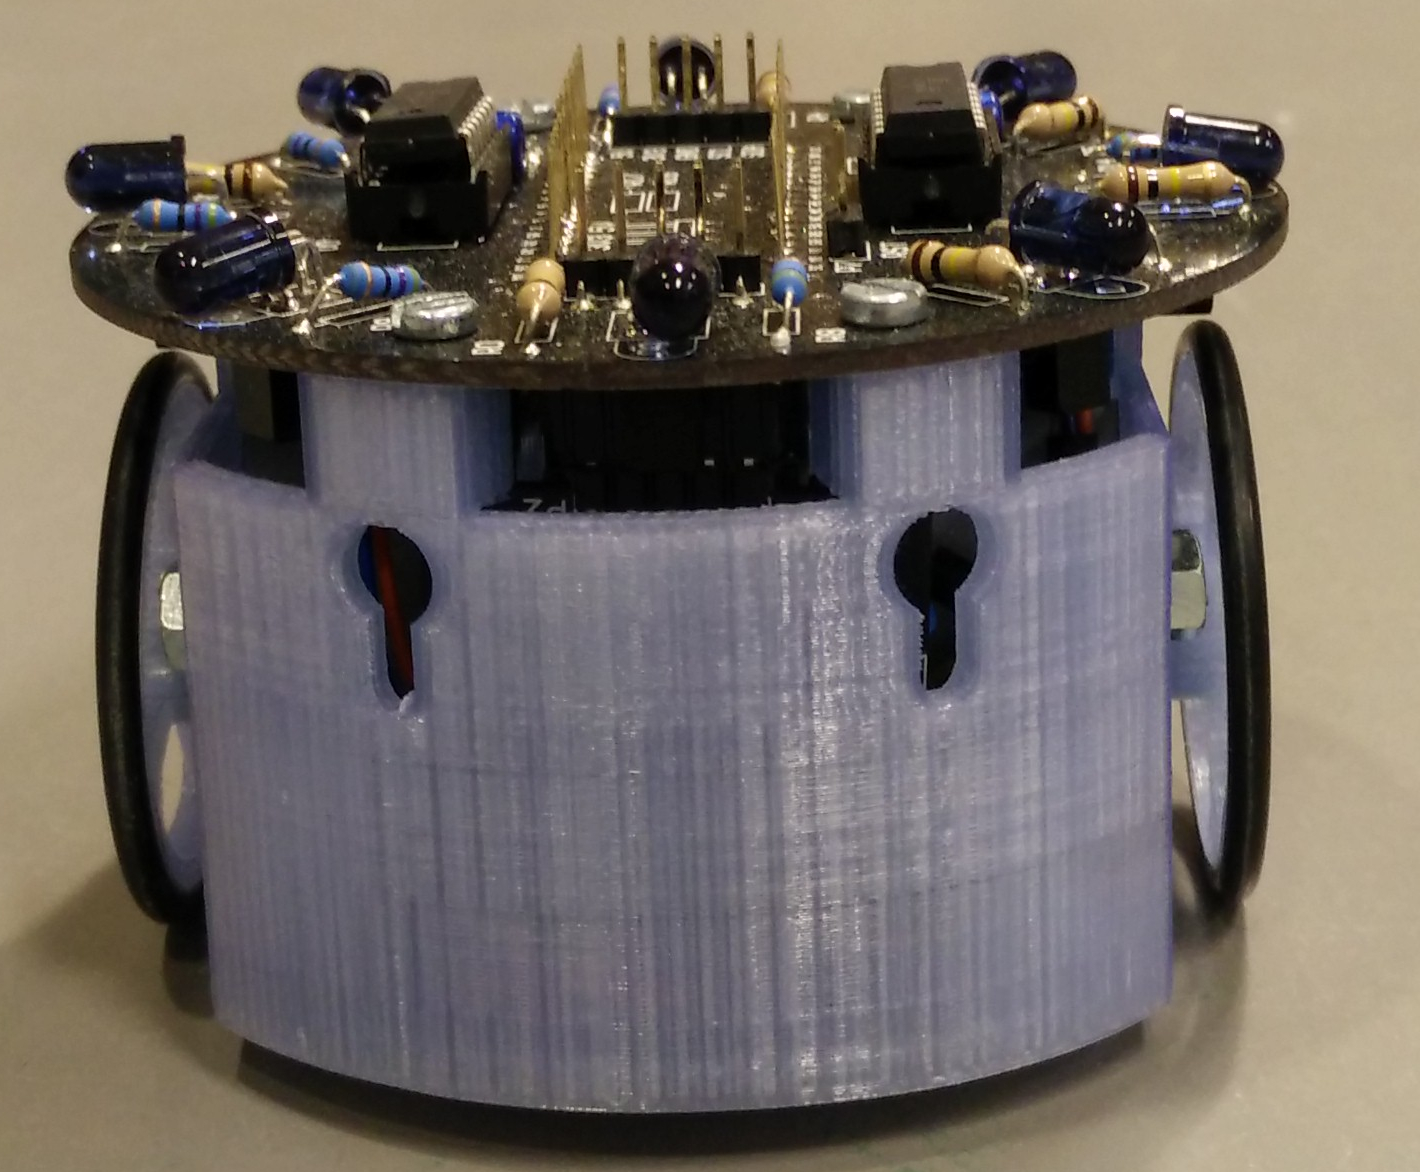
\includegraphics[width=0.8\linewidth]{images/chirpFront.jpg}
\caption{The front of the ChIRP robot}
\label{fig:chirpsFront}
\end{figure}
The purpose behind the development of the ChIRP robot is to research sub symbolic AI, whether it is swarming or evolution. Sub symbolic AI are algorithms and AI inspired by nature or biology. This covers Artificial Neural Network inspired from the human brain, swarm robots inspired from bird flocks, ant colonies, fish schools etc. Evolution and genetic programming are also one of topics included in sub symbolic AI.
The robots' data schema and source code are all open source and can be found at \href{http://chirp.idi.ntnu.no}{chirp.idi.ntnu.no}. The robot consist of a printed circuit board (PCB) which can be seen on "REF", 2 motors which controls the 2 wheels on each side of the robot.
Modules like LED lights and various sensors can be soldered on the PCB thus the robots' are easily modifiable, and the robots can have multiple layers with different sensors so it's not limited to have only light sensors or IR sensors. The standard ChIRP robot comes with 8 infrared-LEDs and 8 infrared receivers as seen on figure \ref{fig:chirpAbove}.
\begin{figure}[H]
\centering
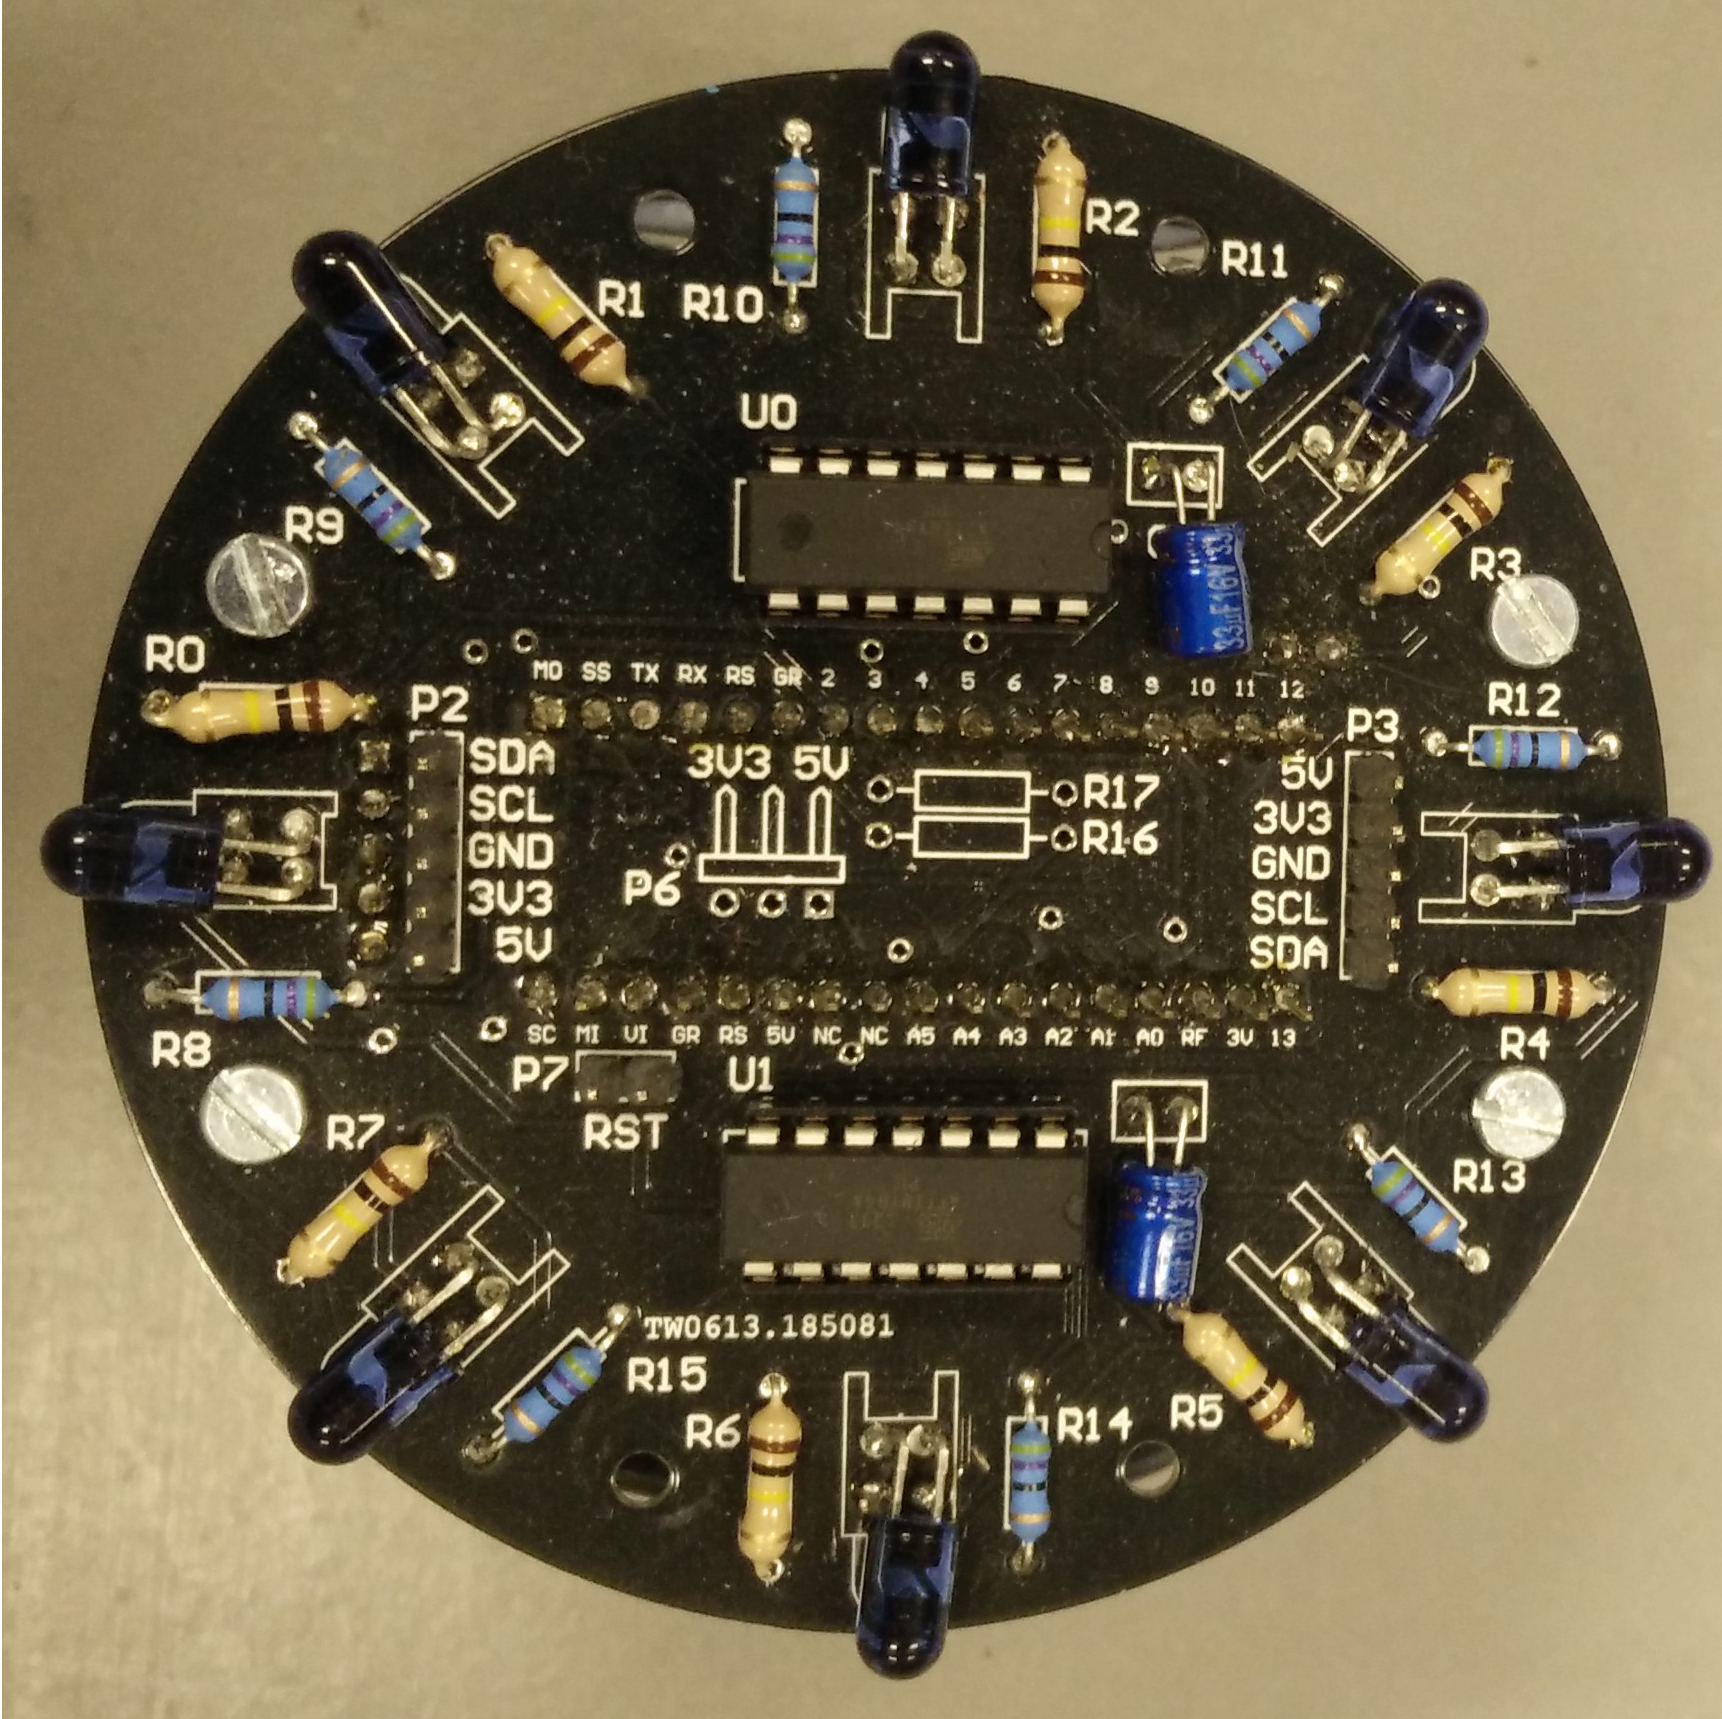
\includegraphics[width=0.8\linewidth]{images/chirpAbove.jpg}
\caption[ChIRP robot seen from above]{ChIRP robot seen from above, this one is equipped with 8 IR emitter and receivers}
\label{fig:chirpAbove}
\end{figure}
These can be used to measure distance by emitting the IR light and measure how much is reflected back into the receiver. There are 2 Shift registers ICs on top of the PCB, these shift registers handles the values found by the IR receivers and converts them to a short (the datatype, 16 bit int) so the arduino micro inside the ChIRP doesn't need to handle everyting. This is due to the limited processor power of the Arduino micro which has a ATmega32u4 processor with 16 MHz clock speed and 32 KB flash memory. Arduino micro has 20 digital inpput/output (I/O) pins in which 7 of them are PWM, and 12 analog input pins. PWM stands for Pulse-width modulation \footnote{\href{http://arduino.cc/en/Tutorial/PWM}{http://arduino.cc/en/Tutorial/PWM}}, and those pins with PWM are able to emulate analog output by 
Inside the robot there's an ATtiny as well that helps the Arduino control the motors.  
\begin{figure}[H]
	\centering
	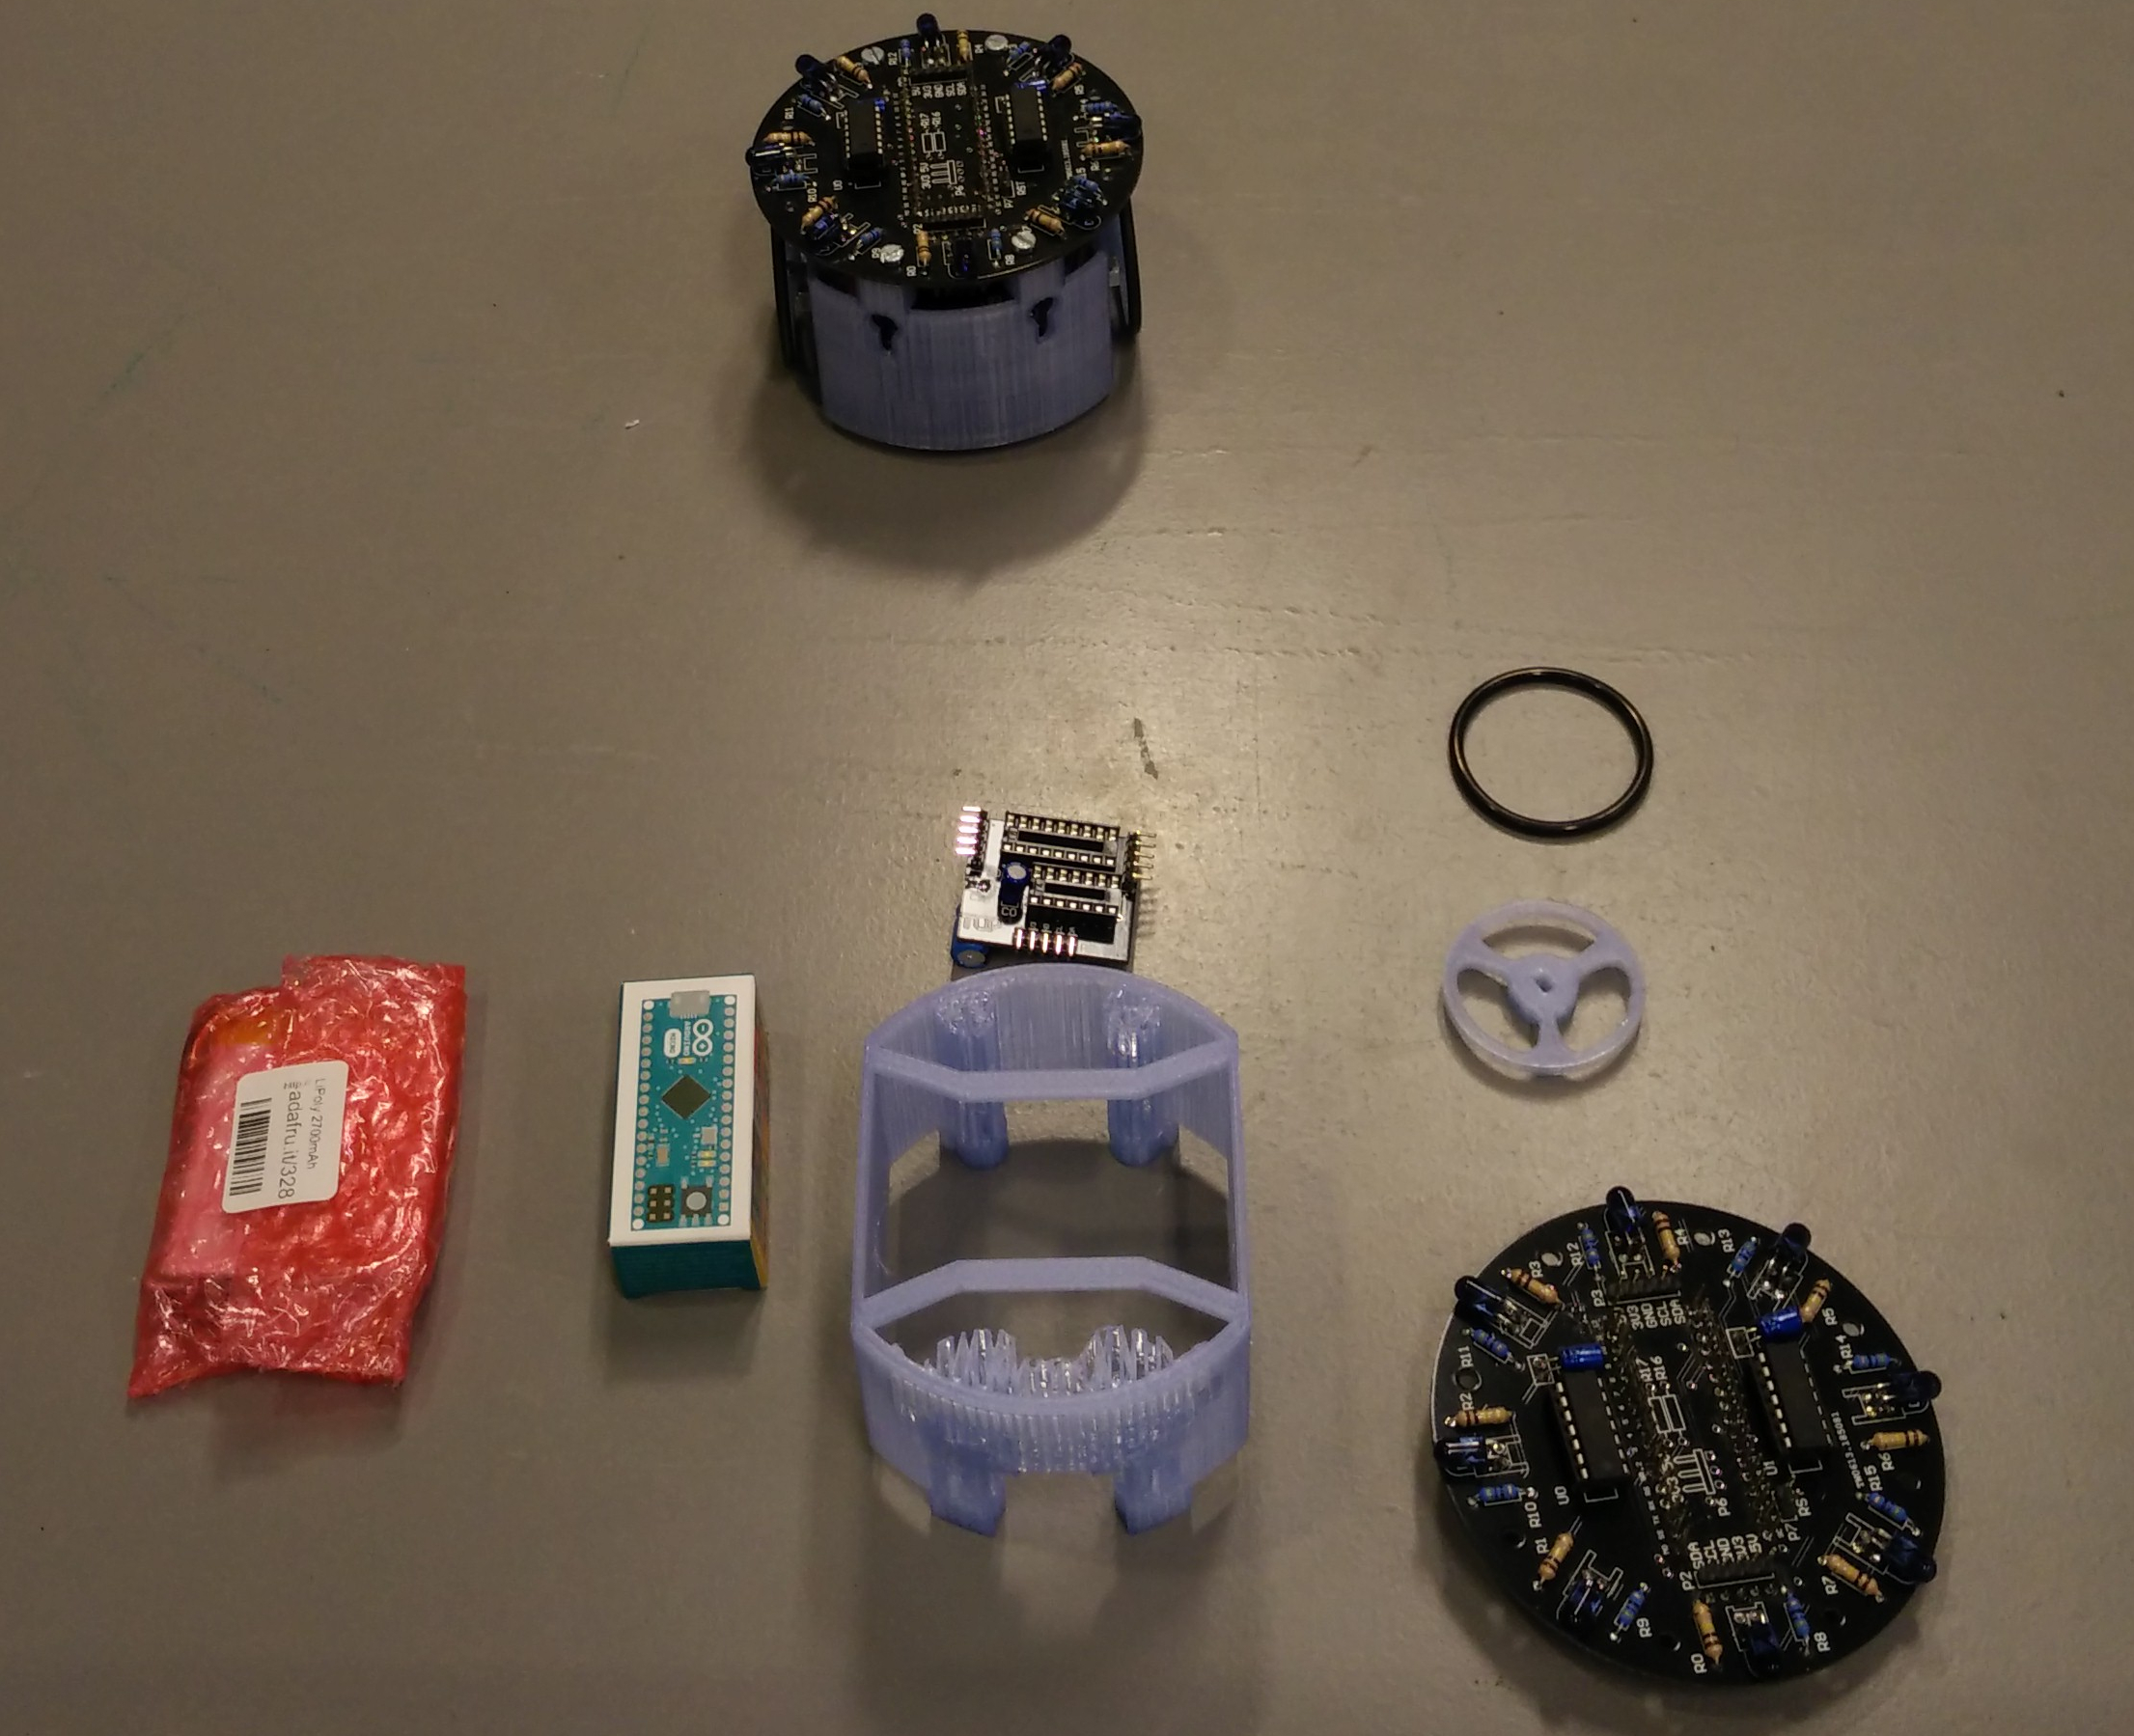
\includegraphics[width=0.8\linewidth]{images/chirpPieces}
	\caption[ChIRP pieces]{The building blocks of the chirp robot}
\end{figure}


The ChIRPs are powered by a 3.7 volts 2500mAh battery which lasts for 4.5 hours if they are running continuously, and it takes around 4 hours to recharge. The battery life can be increased if the robot is standing still. The batteries can be changed, but it can be quite difficult to do so due to the small gaps and the precision needed to connect the wires.

- All code and schemes are available on chirp.idi.ntnu.no
- PCB (printed circuit board)
- Wheels
- 2 motors
- 8 infrared emitters and receivers used for distance measuring.
- Arduino Micro microcontroller.
- Atmel chips to reduce computing on the arduino
- Modules can be added as needed.
- Blueetotth module.
- Other micropchips can be used instead.
- Battery lasts for 4.5 hours, 4 hours to charge.

